\section{Introduction}
In this chapter will be presented the architecture of CPIM especially for the NoSQL service as it was before this work, then will be explained how was possible to include Kundera as persistence layer for the NoSQL service in CPIM and what problem has been faced during the process.
Furthermore in section \ref{sec:hegira} is shown how the integration with the migration system \textit{Hegira} has been introduced, what are the feature supported by this integration and which design choices has been put in place. 

\section{CPIM architecture}
To be able to expose a common interface for the multiple services supported by the library, CPIM adopts heavily the factory and singleton patterns.

\noindent The main access point of the library is the \texttt{MF} (Manager Factory) a singleton object which is responsible of reading the configuration files and exposing a set of methods that will build instances for the service factories.
The initialization is done through the first call to \texttt{MF.getFactory()} which read the configuration files and build an instance of \texttt{CloudMetadata} which will be referenced by all the other services and contains all the information stored in the configuration files.
 
\newparagraph The library is organized in several packages each of one is responsible of a particular service.
\noindent Each service exposes a factory class which is invoked through the \texttt{MF} factory, the service factory maintains a singleton instance of the provider-specific service implementation which is built at the first call based on the configuration available inside the singleton instance of \texttt{CloudMetadata}.
The result of this process is that with the same method call, based on the configuration file, is instantiated one service implementation or another.

\subsection{NoSQL service}
Before this work CPIM library supports NoSQL interaction through Java Persistence API.
The interoperability with the supported clouds is made possible thanks to the previously described factory pattern, a complete class diagram for this service can be seen in the figure \ref{fig:cpim-nosql}.

\begin{figure}[tbh]
  \centering
  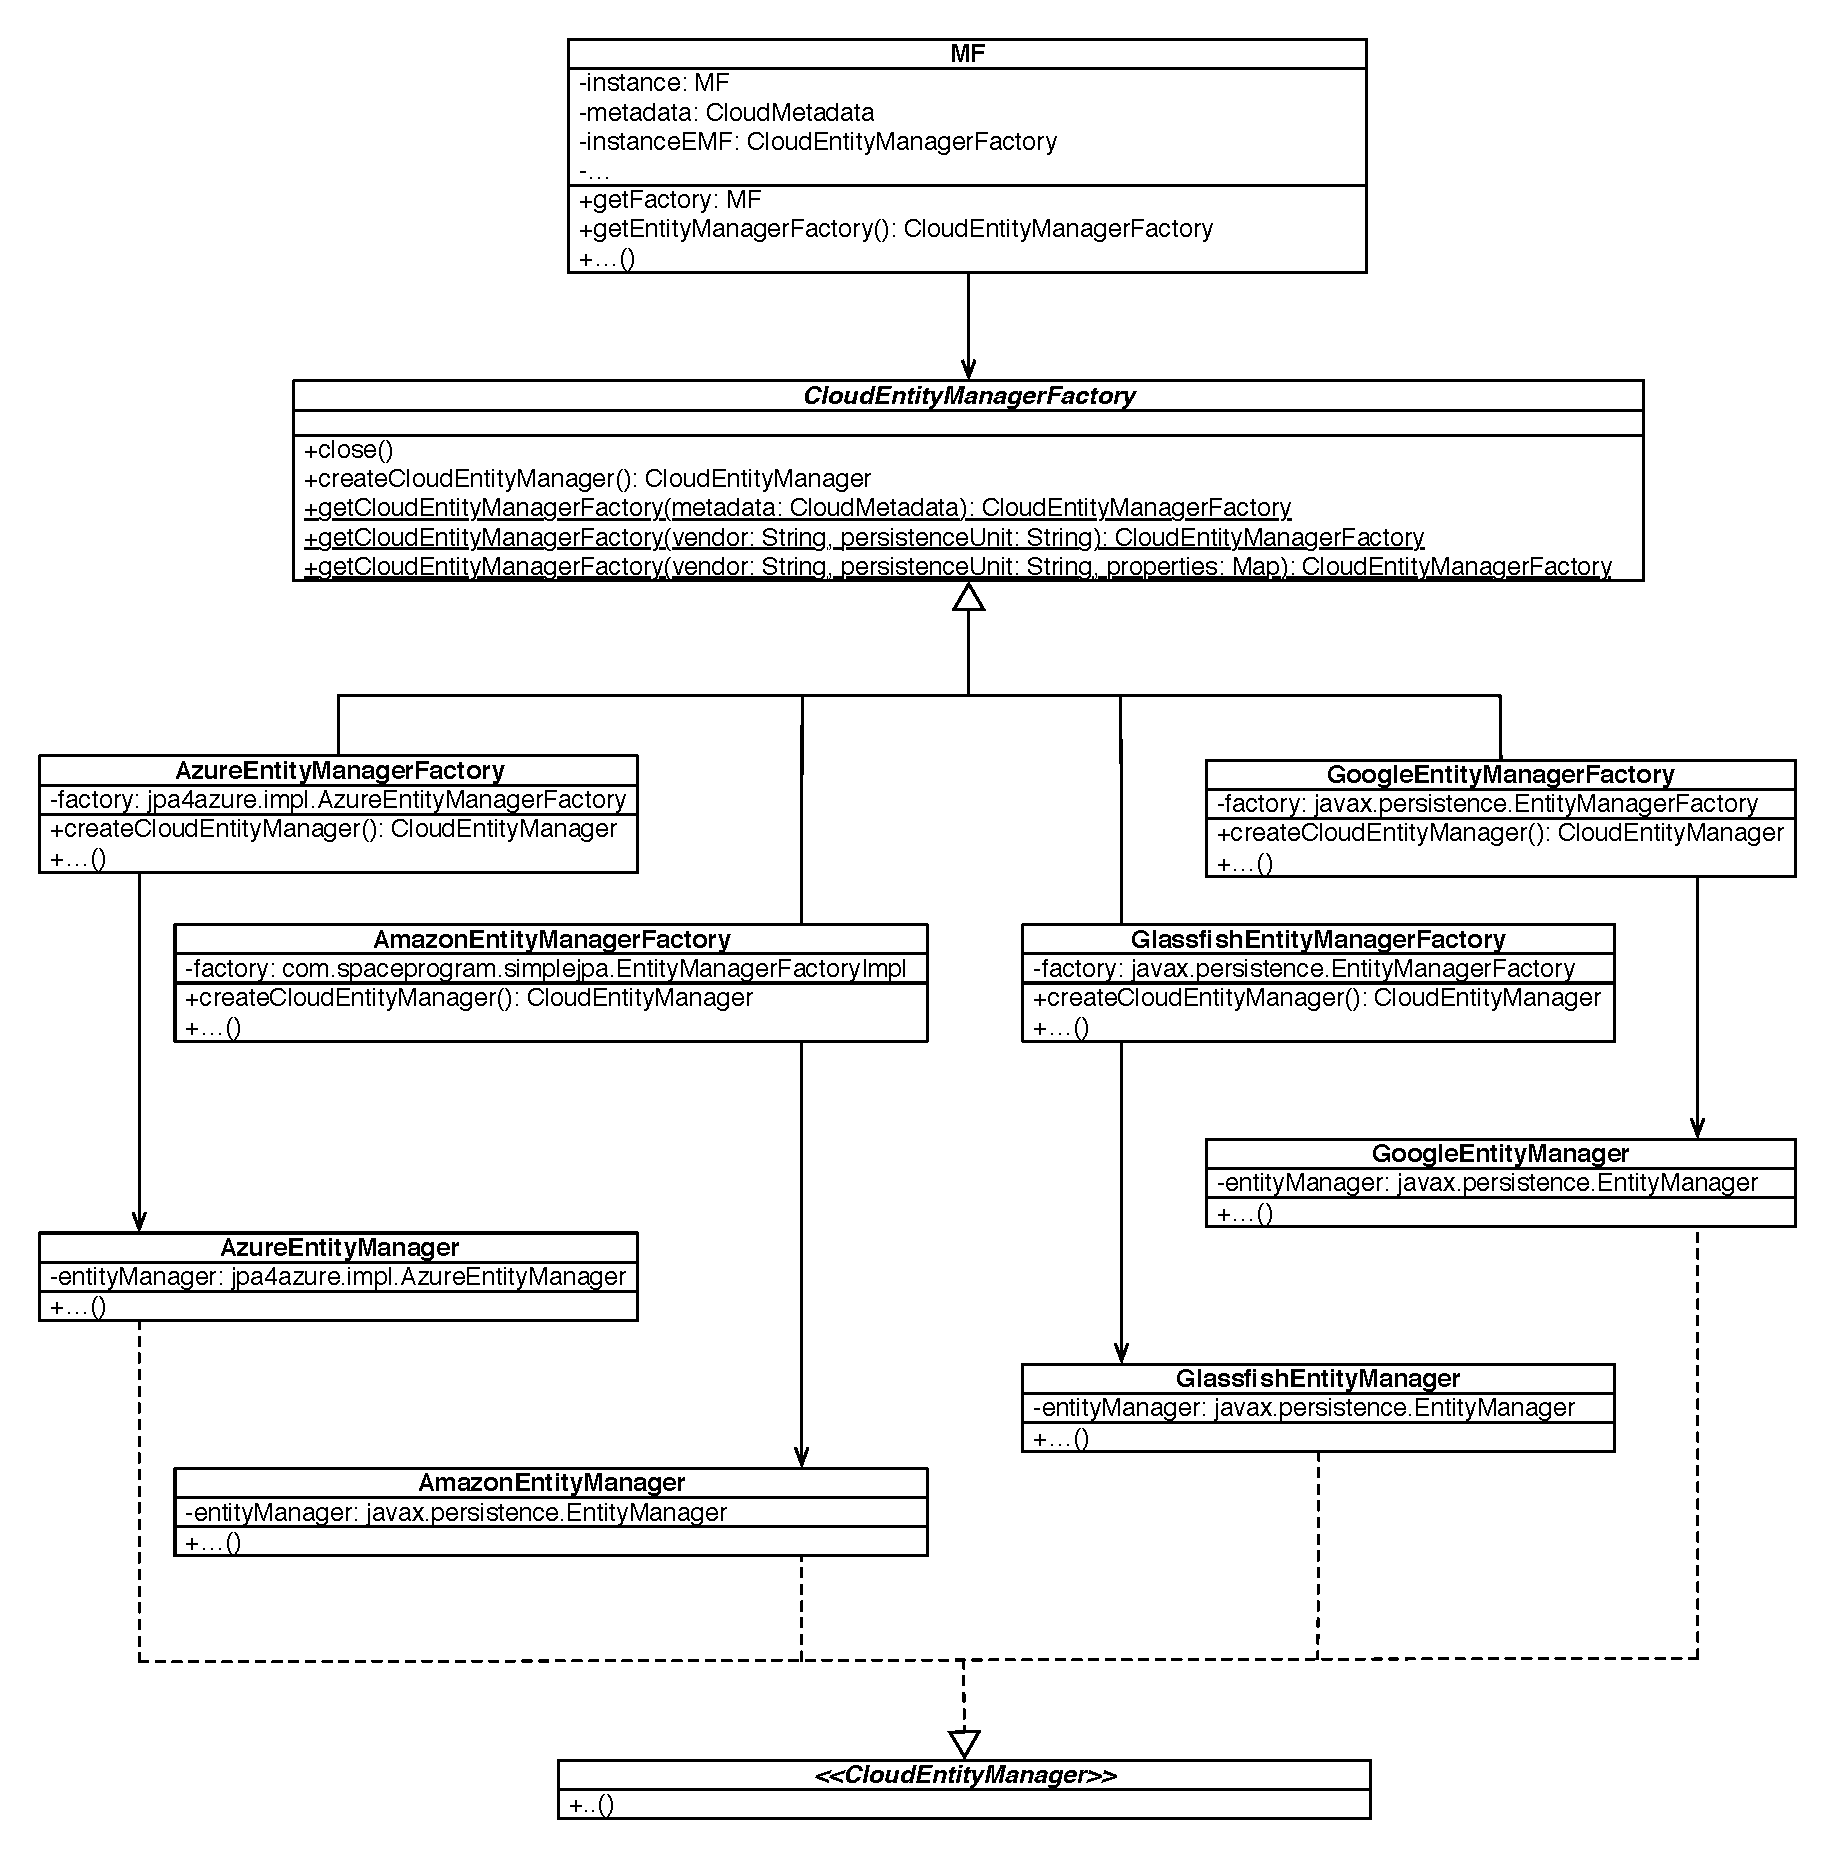
\includegraphics[width=14cm]{images/cpim_nosql_old}
  \caption{NoSQL service architecture}
  \label{fig:cpim-nosql}
\end{figure}

\noindent To use the service, the first step is instantiate a \texttt{CloudEntityManagerFactory} and, depending on the configuration file, this factory instantiate the vendor specific factory. For example in case that Google is the chosen vendor, the instantiated factory will be \texttt{GoogleEntityManagerFactory}. 
Each provider-specific \texttt{EntityManagerFactory} is responsible of instantiating an \texttt{EntityManager} which is the gateway to the underlying database. All the vendor-specific \texttt{EntityManager}(s) implement the common \texttt{CloudEntityManager} interface to achieve uniformity in methods and behavior.
The various implementation of the \texttt{CloudEntityManager} delegates every method call to the vendor-specific persistence provider. 

\newparagraph JPA is not a default language for NoSQL (as described in chapter \ref{chap:sota}) but, due to its wide usage among Java developers, several JPA implementation has been build upon various NoSQL databases both developed by the vendor of the NoSQL storage or by the community.
This means that to support the NoSQL service through the JPA interface, an implementation of the JPA interface must be found. There are so three different persistence providers, one for each cloud provider:
\begin{itemize}
\item for \textit{Google Datastore} its used an official JPA implementation, available inside the SDK
\item for \textit{Amazon SimpleDB} its used \textbf{SimpleJPA}, a third-party implementation of the JPA interface
\item for \textit{Azure Tables} its used \textbf{jpa4azure}, a third-party implementation of the JPA interface
\end{itemize}

\noindent There are couple of things to notice: Amazon SimpleDB has been deprecated in favor of DynamoDB and \textit{jpa4azure} is not being maintained anymore, therefore CPIM needs to be updated in order to get rid of those outdated software.

\section{Kundera integration}
To solve this problems and reduce the number of software on which the CPIM rely on to provide the NoSQL service, the proposed solution  to modify the current CPIM architecture with a unique persistence provider that has been identified in Kundera.

\newparagraph The proposed solution is resumed in the architecture of figure \ref{fig:cpim-kundera} in which the benefit of having a single JPA provider are clearly visible. The architecture is slightly less articulated and no check on the selected provider is needed since this is handled by Kundera while reading the \texttt{persistence.xml} file in which the user will define what datastore is interested in.
Another benefit of this architecture is that the choice of the NoSQL technology is no more bound to the vendor specified in the CPIM configuration file, is in fact possible deploy the application in one of the supported PaaS provider and choose as NoSQL solution of another one which will be addressed remotely, simply by configuring the \texttt{persistence.xml}, moreover it's possible exploiting the Kundera polyglot persistency, to persist part of the data in a database and another part in another one defining the persistence units properly.

\begin{figure}[tbh]
  \centering
  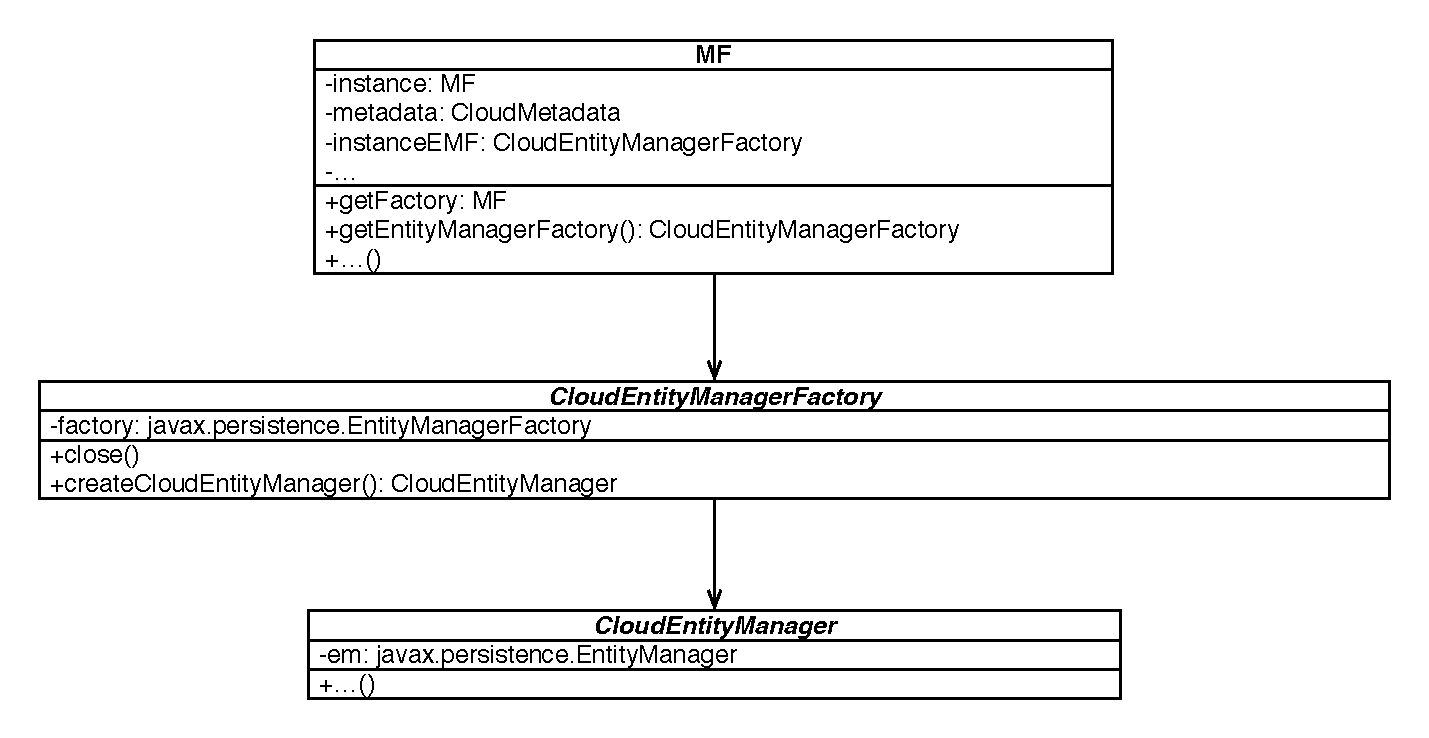
\includegraphics[width=14cm]{images/cpim_nosql_kundera}
  \caption{The modified NoSQL service architecture}
  \label{fig:cpim-kundera}
\end{figure}

\noindent The actual implementation is completely provider agnostic in the sense that actually Kundera is not required as dependency and in fact is not listed as a dependency for CPIM. At run-time, when a Kundera client will be listed in the dependency of the user application, as well as CPIM, the persistence provider dependency will be satisfied.
This is due to the fact that the \texttt{CloudEntityManagerFactory} and the \texttt{CloudEntityManager} implements respectively the JPA interfaces  \texttt{EntityManagerFactory}  and \texttt{EntityManager}.
The actual call to the runtime provider is within the \texttt{CloudEntityManager} that on construction instantiate an instance of the provider \texttt{EntityManager} and uses that reference to delegate every method execution to it.

\noindent This can seems a over-designed architecture but it turns out to be extremely necessary in order to provides a transparent interaction with the migration system as it will explained later on in this chapter.

\subsection{Problems encountered}
Kundera provides an uniform access through the JPA interface independently from the provider, which is somehow defined in the \textit{persistence.xml} through the Kundera client selection. For this reasons all the old libraries that provides a JPA implementation for a specific provider can be removed from the CPIM. 
This tentative in cleaning the dependency of CPIM caused two main problems:
\begin{enumerate}
\item \textit{jpa4azure} turns out to be used also for Queue and Blob service of Windows Azure
\item Kundera seems to have problem when multiple persistence provider are found in the classpath and has not be found a way to force the selection of Kundera as persistence provider (besides specifying it in the \textit{persistence.xml} file)
\end{enumerate} 

\noindent To solve the first problem, the code of the extended version of\textit{jpa4azure} has been inspected since it was extended to support some missing functionalities of the JPA interface, the library contains two main packages:
\begin{itemize}
\item \texttt{jpa4azure}, which contains the code that implement the JPA
\item \texttt{com.windowsazure.samples}, which contains the code do ease the communication with the Azure services
\end{itemize}
The \texttt{jpa4azure} package has been removed and the library rebuild since the other package is the one used in the Blob and Queue service. Its possible to completely remove \texttt{jpa4azure} but is necessary to rewrite also the CPIM Blob storage service for Azure using the Azure SDK.

\newparagraph CPIM shows more errors in the code in the Queue service and after some investigations, turns out that when \textit{jpa4azure} was extended the class \texttt{AzureQueueManagerFactory} and other were introduced.
The problem was that \texttt{AzureQueueManagerFactory} use the JPA interface to communicate with the Queue service so removing the support to JPA interface has leaded to lose the support to Azure Queue service.
One possible solution to this would be rewrite the CPIM Queue services for Azure using Azure SDK.

\section{Hegira integration}
\label{sec:hegira}
To support data synchronization and migration, the NoSQL service was further modified to integrate with \textbf{Hegira} \cite{thesis:marco}. An high level schema of the interaction we want to achieve is reported in figure \ref{fig:high-level-interaction}

\begin{figure}[tbh]
  \centering
  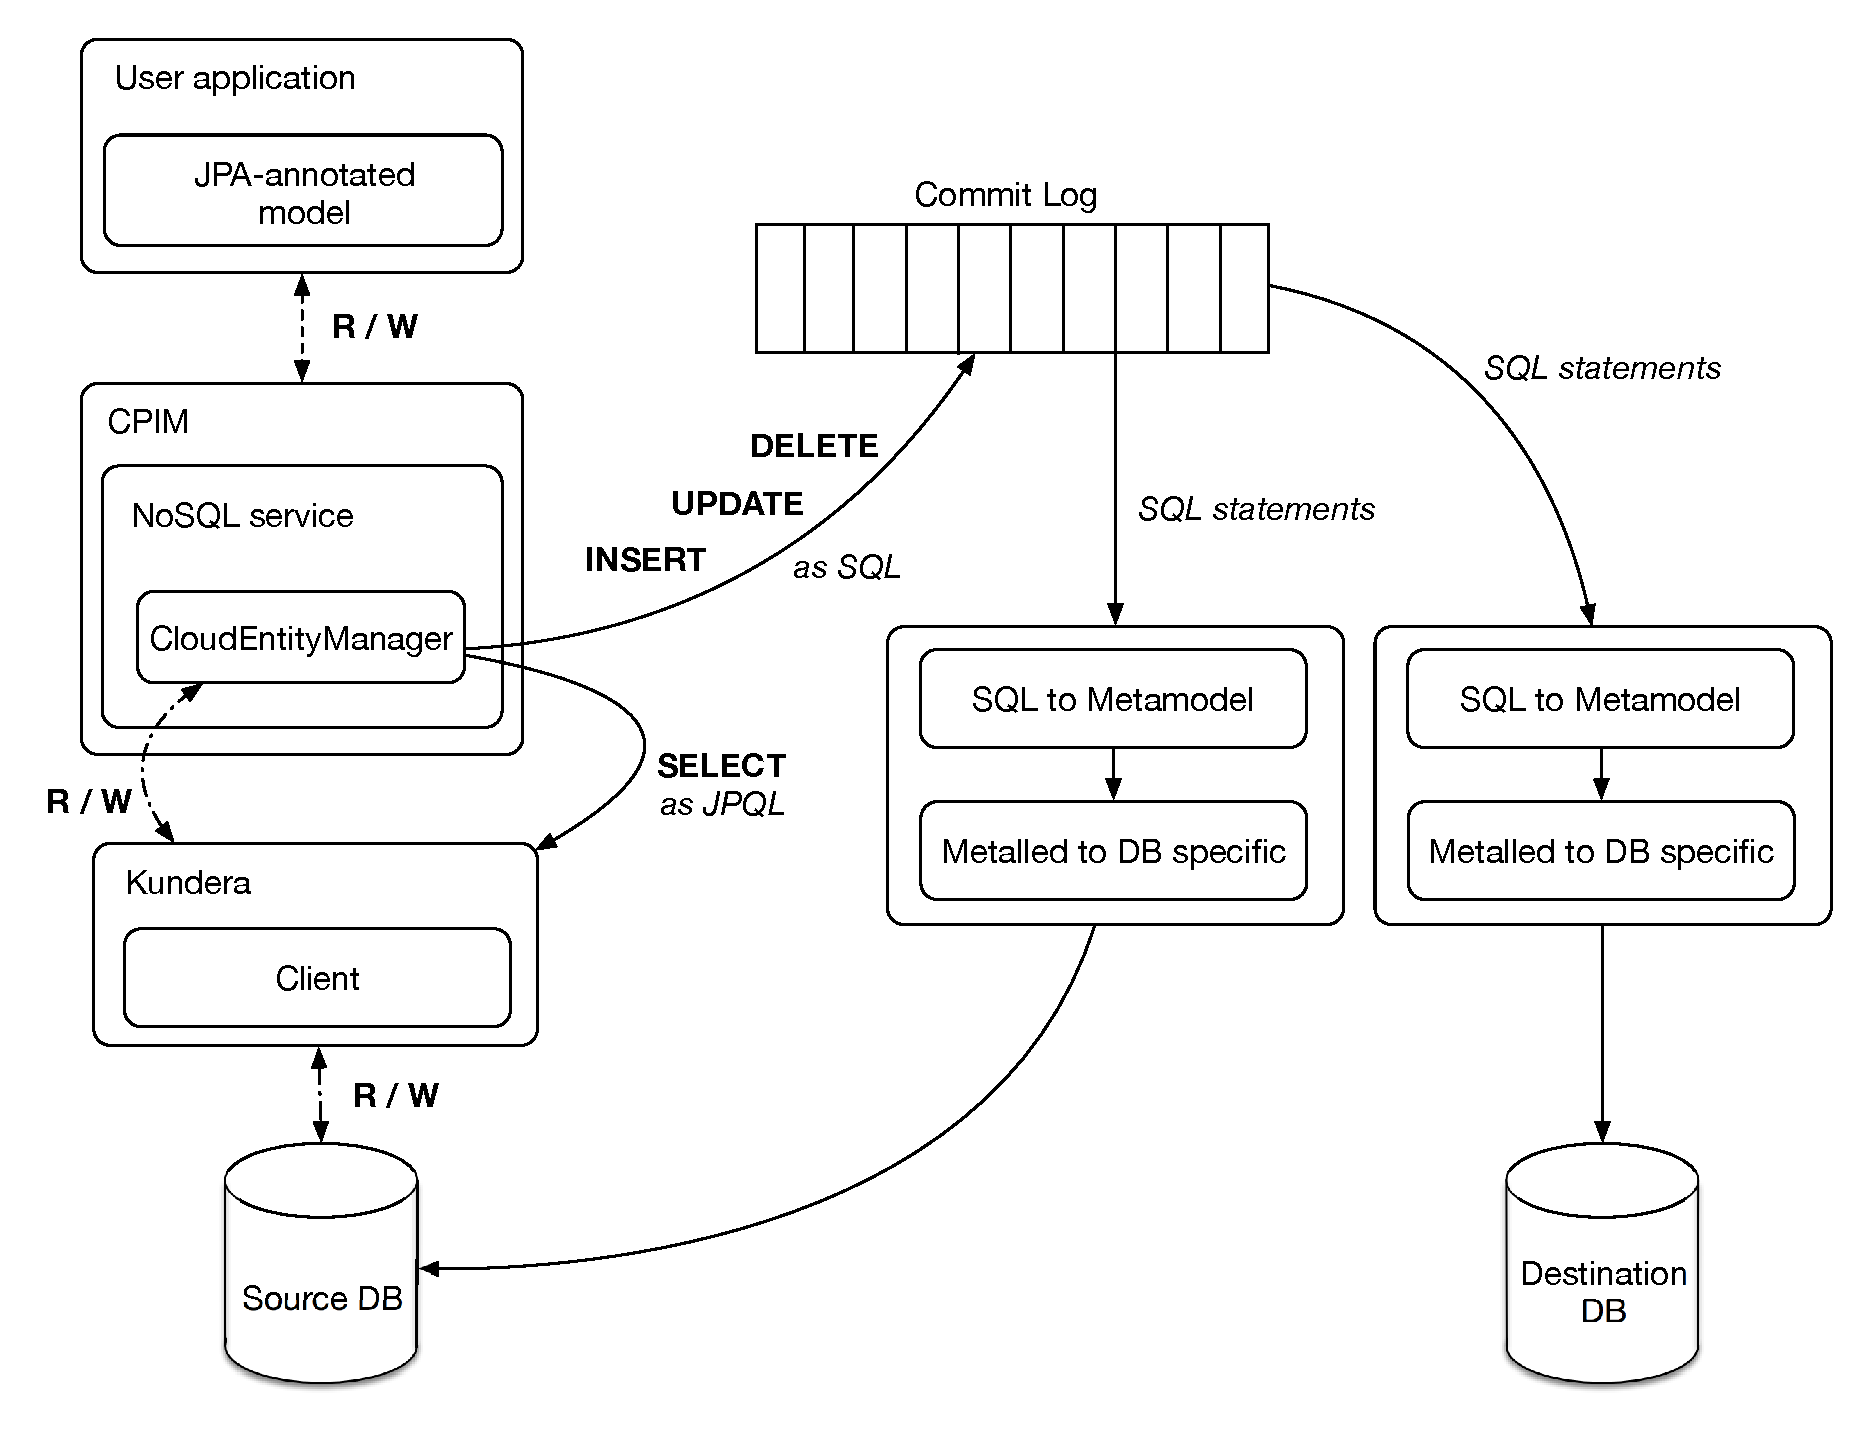
\includegraphics[width=12cm]{images/high_level_interaction}
  \caption{High level schema of interaction}
  \label{fig:high-level-interaction}
\end{figure} 

\noindent In the above schema, \textit{dashed} lines represents the normal flow of data from the user application to the local database, the filled ones represents the behavior in case a migration is in process and so the local database is bypassed. CPIM library needs to connect to the migration system in order to understand when migration is in progress and in that case only bypass the interaction with Kundera by building a string representation of the user operation in a SQL format, then this string is sent to the commit log of \textit{Hegira} that then will pop the statements and translate those SQL statement into a datastore-specific operation.

\subsection{Migration Manager}
Interaction with the migration system is handled primarily by the \texttt{MigrationManager} class which follows a state pattern represented in the class diagram \ref{fig:migration-class-diagram}. 
 
\begin{figure}[tbh]
  \centering
  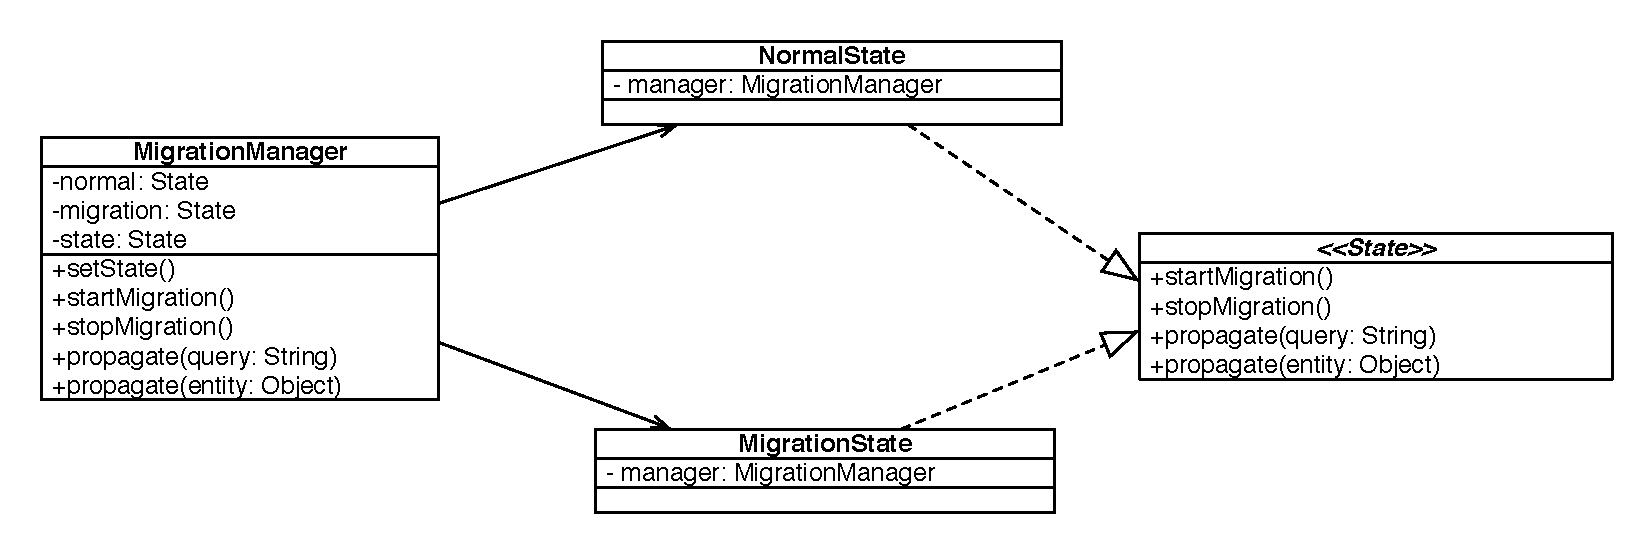
\includegraphics[width=14cm]{images/migration_class_diagram}
  \caption{\texttt{MigrationManager} class diagram}
  \label{fig:migration-class-diagram}
\end{figure} 

\noindent The pattern permits to the \texttt{MigrationManager} to delegates the method execution to the current state, the state diagram is the one represented in figure \ref{fig:migration-fsa} is and composed by two states \texttt{Migration} and \texttt{Normal} that encapsulate the required behavior.
    
\begin{figure}[tbh]
  \centering
  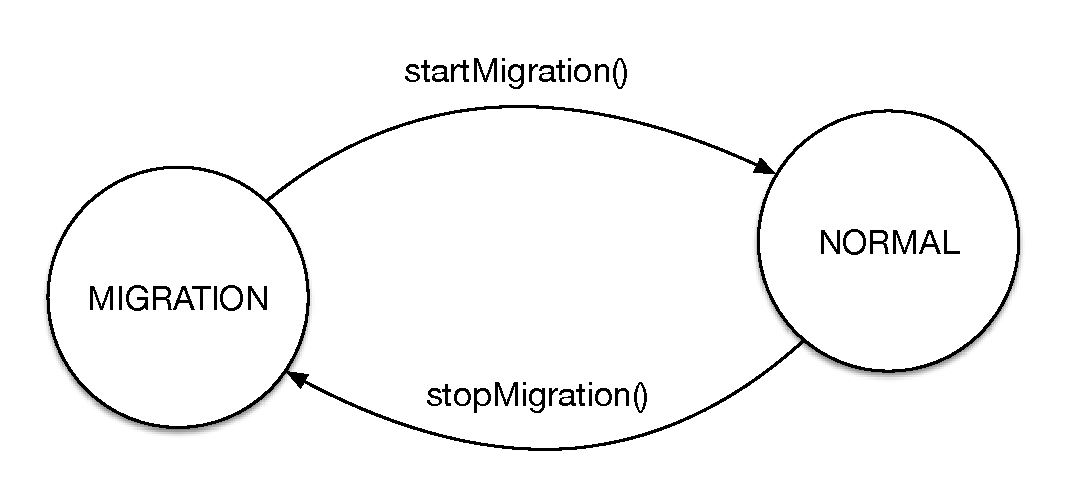
\includegraphics[width=6cm]{images/migration_fsa}
  \caption{\texttt{MigrationManager} states}
  \label{fig:migration-fsa}
\end{figure} 

\noindent This part of the design was actually made before knowing exactly how the interactions will exactly be since the component to interact with were not finished yet. Hence in order to have a well-defined place in which behavior has to be encapsulated, the state pattern was the best solution even for future extensibility in case the interaction with the migration system will become more complex.  

\section{Intercept user operations}
The first operation that needs to be analyzed is where is possible to intercept user operation is a way that is completely transparent to the user.
The operation that we want to intercept are the insert, update and delete operation cause those are the operation that alter the structure of the data and thus are the one that needs to be processed by the migration system.

\subsection{Intercepting CRUD operations}
CRUD operation are always handled in the \texttt{EntityManager}, three are the methods that needs to be intercepted:
\begin{itemize}
\item \texttt{EntityManager.persist(Object entity)} for the insert operation
\item \texttt{EntityManager.merge(Object entity)} for the update operation
\item \texttt{EntityManager.remove(Object entity)} for the delete operation
\end{itemize}
\noindent User is not directly invoking method on the provider entity manager but interacts with the persistence provider through the \texttt{CloudEntityManager} class. Without the support for the migration system the \texttt{CloudEntityManager}, as stated previously, delegates every method call to the provider entity manager.
To integrate migration and synchronization logic, the methods mentioned above should contain a little more amount of logic shown in the snippet of code \ref{code:isMigrating} taking as example the update operation.

\begin{lstlisting}[language=Java, caption=Integrate migration logic, label=code:isMigrating]
public <T> T merge(T entity) {
    if (MigrationManager.isMigrating()) {
        MigrationManager.propagate(entity, OperationType.UPDATE);
        return entity;
    } else {
        return delegate.merge(entity);
    }
}
\end{lstlisting}

\noindent In case of migration is visible the call to the \texttt{propagate} method. It accept two arguments:
\begin{itemize}
\item the entity to be converted to a statement
\item the operation that needs to be generated
\end{itemize}
The method is called on the \texttt{EntityManager} which then delegates the execution to the current state which should be the migration state at that point. The \texttt{propagate} method of the migration state is responsible of building the requested statements using the statement builders and then sending the generated statements to the commit log of \textit{Hegira}. Both action are described in detail later on.

\subsection{Intercepting queries}
A first look at the JPQL specification \cite{book:projpa2} revealed that JPQL does not support \textit{INSERT} statements and so the only way user have to persist entities is through \texttt{EntityManager.persist(Object entity)} that is one of the case described in the previous section, so only the remaining cases (\textit{UPDATE} and \textit{DELETE}) needs to be intercepted.

\noindent JPA interface provides several ways to build and execute queries all available by calling the proper methods defined in the \texttt{EntityManager} interface: 
\begin{itemize}
\item \texttt{createQuery} from JPQL query string
\item \texttt{createQuery} from an instance of \texttt{CriteriaQuery}
\item \texttt{createNamedQuery}
\item \texttt{createNativeQuery}
\end{itemize}
 
\noindent Native queries are clearly not supported by Kundera and thus from the migration system clearly because there not so many storage that provides a SQL-like language to specify queries.
Create queries through \texttt{CriteriaQuery} is currently not supported.
The remaining two kind of methods are the supported ones.

\newparagraph JPA does not provide through the \texttt{Query} interface to get the JPQL representation of the query. Queries are supposed to be written as method argument when creating them through the \texttt{EntityManager} or called by name if they are defined as named queries upon some class.
That was actually a problem since in order to be able to parse the query its JPQL representation is crucial.

\noindent The easiest solution was to implement the interfaces for \texttt{Query} and \texttt{TypedQuery} respectively with the classes \texttt{CloudQuery} and \texttt{TypedCloudQuery}. This allows to transparently maintains the JPQL string representation of the query.
The wrapping of the persistence provider queries is performed in the entity manager and is performed in the query creation method  in both the versions that return an instance of \texttt{Query} and \texttt{TypedQuery}. The actual JPA query generation is delegated to the persistence provider then, before returning to the user the result query is wrapped in a \texttt{CloudQuery} that contains the generated query and the string representation of it (used by the provider to build the query).

\newparagraph For named queries things are little trickier since the user create instance of \texttt{Query} or \texttt{TypedQuery} just by giving the query name.
\noindent As can be seen from the code snippet \ref{code:wrap-named-queries}, named queries metadata are maintained inside the \texttt{PersistenceMetadata} class. This class, besides maintaining information about named queries, maintains principally a mapping between table names and their class canonical name (full package plus the class name). The content of this class is built the first time is queried (since is a singleton instance) and does not read directly the  configuration files but reads the \texttt{CloudMetadata} instance that has been modified to include all the required parameters that needs to be read from configuration files. 
Information of table to class mapping is required for statements building and for sequence number handling both described later on.

\begin{lstlisting}[language=Java, caption=Wrap named queries, label=code:wrap-named-queries]
public Query createNamedQuery(String name) {
    String queryString = PersistenceMetadata.getNamedQuery(name);
    Query queryInstance = delegate.createNamedQuery(name)
    return new CloudQuery(queryString, queryInstance);
}
\end{lstlisting}

\section{Data synchronization}
\label{sec:synch}
In the previous section, an overview of the required logic that has been built to integrate \textit{Hegira} was described. Now let's face the problem of synchronization that allows the migration to be performed live.

\noindent A special look needs to be reserved for the insert operation. When the user updates or delete an entity no matter if through the entity manager or through a query, he already knows the identifier of that entity since the insert operation have already persisted the entity into the underlying database and thus generated the identifier.
Since we want to guarantee a synchronization with the migration system, user cannot define its own identifiers but them needs to be assigned from the migration system.
The main caveats is that such assignment has to be made even if the migration is not running yet so the identifier assignment has to be made in two cases:
\begin{enumerate}
\item insert statements built from persist operation during a migration phase
\item \textit{standard} insert operation through the entity manager during a normal state
\end{enumerate}

\noindent The solution is actually quite simple since everything can be checked inside the \texttt{EntityManager.persist} method as described in the snippet of code \ref{code:persist}.

\begin{lstlisting}[language=Java, caption=Persist operation, label=code:persist]
public void persist(Object entity) {
    if (MigrationManager.isMigrating()) {
        MigrationManager.propagate(entity, OperationType.INSERT);
    } else {
        String tableName = ReflectionUtils.getJPATableName(entity);
        int id = SeqNumberProvider.getNextSequenceNumber(tableName);
        ReflectionUtils.setEntityId(entity, id);
        delegate.persist(entity);
    }
}
\end{lstlisting}

\noindent In the code snippet is visible a call to the  \texttt{SeqNumberProvider} class which is the class responsible of actually interacts with the synchronization service of Hegira and handle the \textit{sequence numbers} i.e. the entities identifiers defined by Hegira to achieve synchronization. 

\subsubsection{Handling the sequence numbers}
The sequence numbers are handled by the class \texttt{SeqNumberProvider}, a singleton instance that provides a simple way to get the assigned sequence numbers per table.
\noindent The class diagram of this component and of the component it interacts with is shown in figure \ref{fig:seq-provider}

\begin{figure}[tbh]
  \centering
  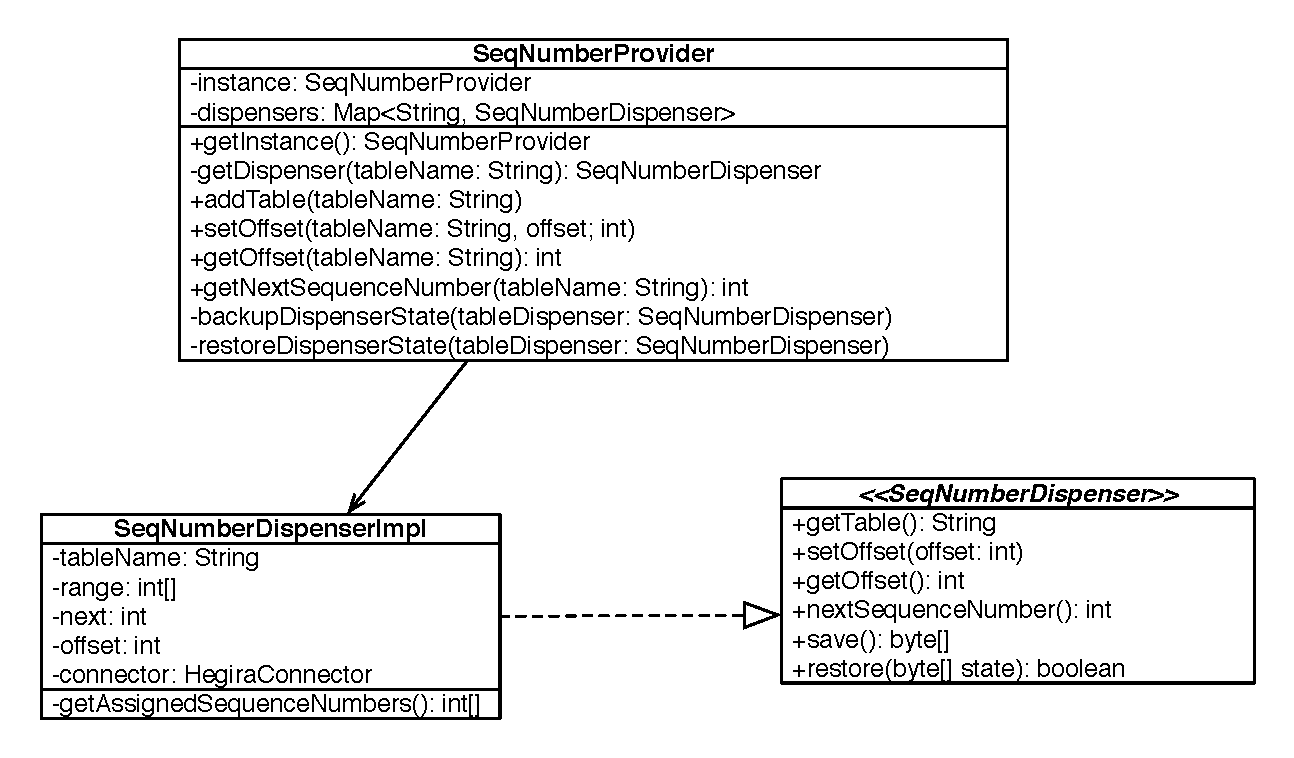
\includegraphics[width=12cm]{images/seq_provider}
  \caption{Sequence numbers handling architecture}
  \label{fig:seq-provider}
\end{figure} 

\noindent The \texttt{SeqNumberProvider} keeps an instance of \texttt{SeqNumberDispenser} for each table that needs to be persisted and is responsible of:
\begin{enumerate}
\item provide a unique access point where requesting the next assigned sequence number for a table
\item initialize or restore the state of the dispenser for each of the persisted tables
\end{enumerate}
\noindent The first is performed through the method \texttt{getNextSequenceNumber(String tableName)} that delegates the operation to the correct \texttt{SeqNumberDispenser} associated to the requested table.
Since \texttt{SeqNumberDispenser} is an interface, the actual implementation is delegated to the \texttt{SeqNumberDispenserImpl} class, this mechanism has been used to be able, maybe in the future, to create more dispensers with different logic.
\noindent The \texttt{SeqNumberDispenserImpl} class maintains internally the assigned range of identifiers provided by the synchronization system by specifying the first and the last element of the range. The class consumes one by one the identifiers in the range and when the range has been completed requests the next range. This mechanism is internally handled, in fact the \texttt{SeqNumberProvider} is only required to call the \texttt{getNextSequenceNumber()} method on the dispenser.
In case the user wants to have control over the sequence number range for a particular table, it has been made configurable at run-time. At construction time each \texttt{SeqNumberDispenserImpl}  class reads the default range from \texttt{CloudMetadata} but by calling the method \texttt{setOffset(String tableName, int offset)} on the \texttt{SeqNumberProvider}, it will set the specified offset to the \texttt{SeqNumberDispenser} responsible of the given table.

\newparagraph The second functionality is achieved by requesting to the \texttt{SeqNumberDispenser}(s) their state representation (as a \texttt{byte} array) by calling the method \texttt{save()} on the dispensers and then saving it to a Blob storage or to file depending to the configuration specified inside \textit{migration.xml}, described in appendix \ref{app:migration}. 
\noindent The restoring phase is performed just after construction, if a backup exists, either on file or on the Blob storage, the method \texttt{restore(byte[] state)} is called on the dispensers giving them their state representation to restore.
This mechanism in which the \texttt{SeqNumberProvider} is completely agnostic to the actual state representation of the \texttt{SeqNumberDispenser}(s) to make future extensibility more easy and less constrained.
The \texttt{SeqNumberProvider} requests to \texttt{SeqNumberDispenser}(s) their sta

\noindent The list of all the tables to be persisted is retrieved from the \texttt{PersistenceMetadata} mentioned previously for named queries.
 
\subsection{Contacting the synchronization system}
The interaction with the synchronization system as now was only described as a method call. Those calls are made on an external library (\texttt{zkWrapper}) that connects to a zookeeper instance to communicate with the synchronization system and receive the assigned sequence numbers.
Since the zookeeper library issues threads to handle communication, was not possible to use this method for Google App Engine since the App Engine run-time does not permit to spawn thread.
Two are the feature that requires to communicate with the synchronization system and so use the \texttt{zkWrapper}:
\begin{itemize}
\item the migration state listener that modify the \texttt{MigrationManager} state accordingly
\item the \texttt{SeqNumberDispenser}(s) that needs to retrieve the sequence number assigned to tables
\end{itemize} 
\noindent The solution adopted was to modify the \texttt{zkWrapper} library to include an API version that handle the calls not by connecting directly to a zookeeper instance but contacting a remote server through some defined API that ultimately interacts with the migration system.

\newparagraph A simple structure has been built to make both the \texttt{MigrationManager} and the \texttt{SeqNumberDispenser}(s) transparent to the type of client that is used to retrieve information from the synchronization system. The architecture is shown in figure \ref{fig:zk-adapter}

\begin{figure}[tbh]
  \centering
  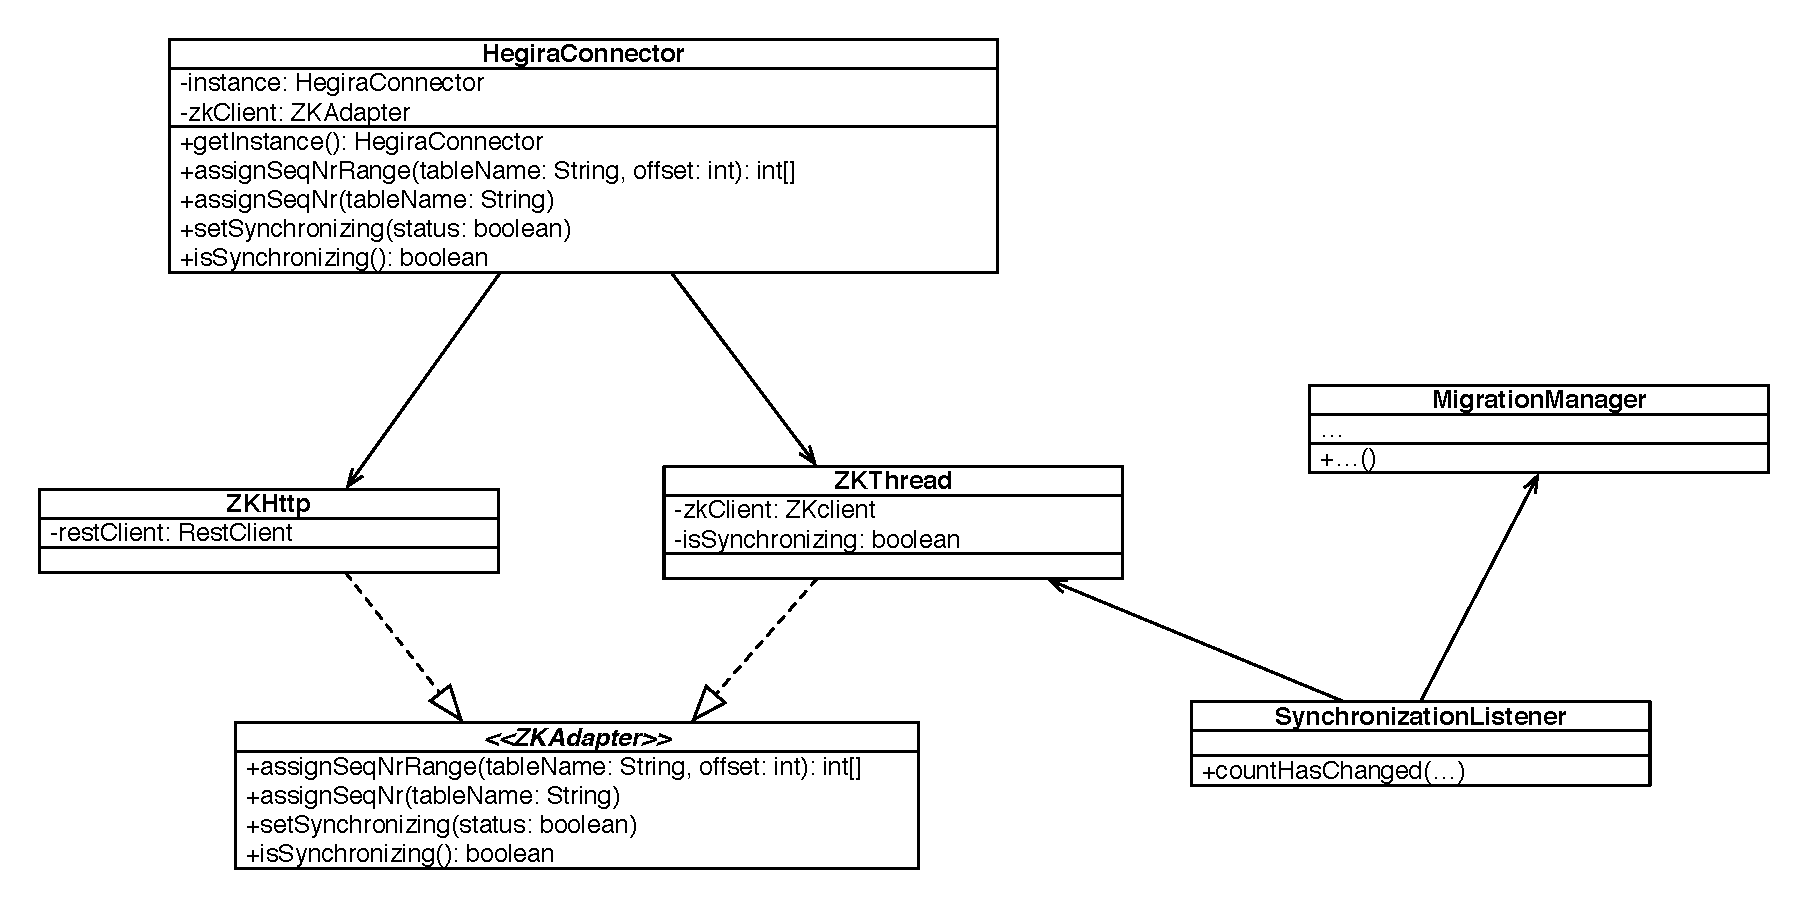
\includegraphics[width=14cm]{images/zk_adapter}
  \caption{Contacting the synchronization system}
  \label{fig:zk-adapter}
\end{figure} 

\noindent The \texttt{HegiraConnector} is the class responsible of deciding which kind of client needs to be instantiated reading the configuration parsed  in \texttt{CloudMetadata}, the \texttt{HegiraConnector}  keeps internally an instance of the instantiated client and provides access to its method by delegation.
The two available clients implements the interface \texttt{ZKAdapter}, built to uniform the methods of the two implementations.

\paragraph{Thread-based client} If the user deploy the application on a thread-capable client and configure the \textit{migration.xml} accordingly, an instance of \texttt{ZKThread} is built. This version of the client uses directly the implementation of the library \texttt{zkWrapper} since there should not be any problem in thread spawning.
The \texttt{isSynchronizing()} methods returns a value which is kept inside the \texttt{ZKThread} instance and is queried by the \texttt{MigrationManager}.
Both the state of the \texttt{MigrationManager} and the value inside \texttt{ZKThread} are modified by the \texttt{SynchronizationListener} which is asynchronously notified by the \texttt{zkWrapper} library when the migration state change.

\paragraph{HTTP-based client} In case that threads are not supported by the cloud provider the client version that is instantiated (by looking at the configuration) is \texttt{ZKHttp} which uses the API-caller added to the \texttt{zkWrapper} library.
Since no listener can be register and asynchronously notified of a change in the migration state and is not possible to somehow cache the state or make assumption on it, each call of the \texttt{MigrationManager} to the method \texttt{isSynchronizing()} will perform an API call to the remote server and will return the state of the synchronization just queried.

\section{Build statements from user operations}
\label{sec:statements}
Before focusing on the statements building, since migration system interaction are getting many, it may be useful to visualize the interaction in the high-level flow chart presented in figure \ref{fig:flow-chart}.

\begin{figure}[tbh]
  \centering
  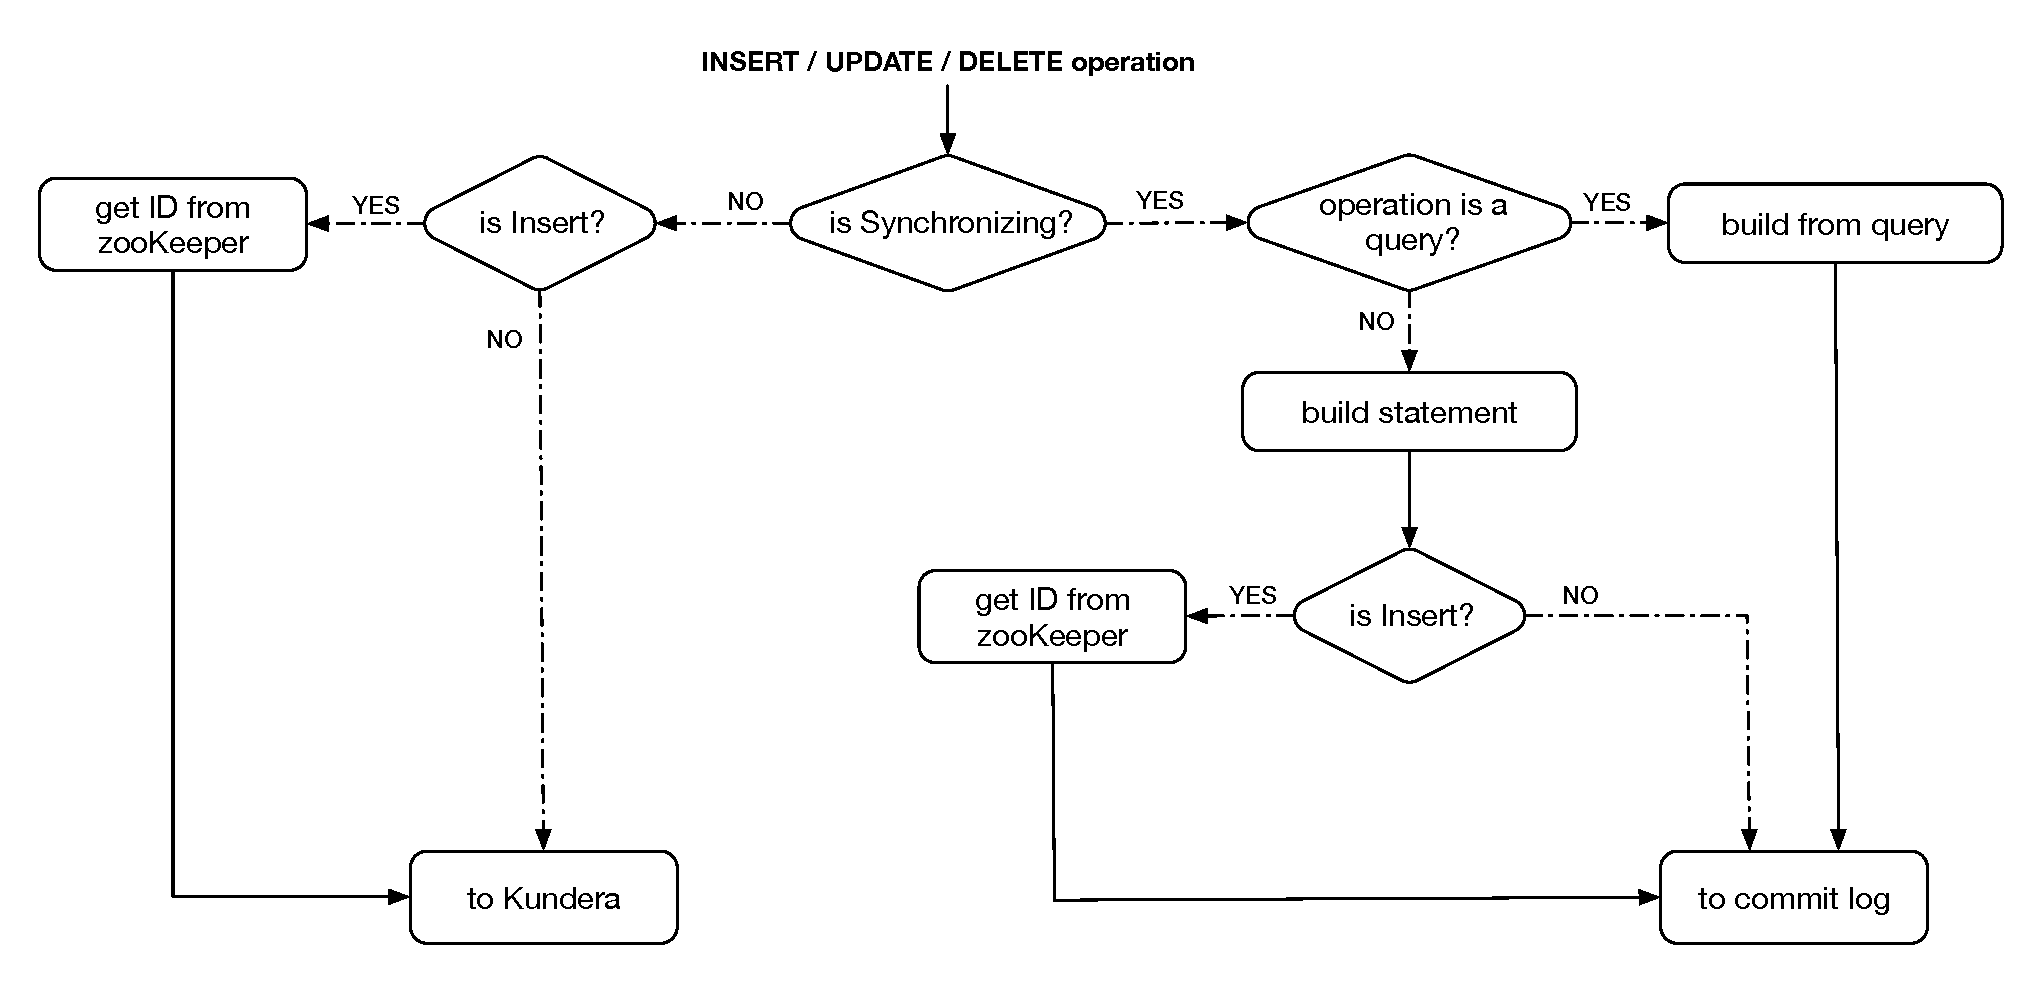
\includegraphics[width=13.5cm]{images/flow_chart}
  \caption{Interaction flow chart}
  \label{fig:flow-chart}
\end{figure} 

\noindent In the previous section we've focused on the sequence number retrieval, in this section we'll focus on the generation of the statements to be sent to \textit{Hegira}.

\newparagraph To be able to create SQL-like statements from queries and operation upon entity objects, the first step has been to introduce the \textit{statement} concept in the library. This has been done through the abstract class \texttt{Statements} that encapsulate the structure needed for maintaining the necessary data for the statements and is  then extended by the three classes \texttt{InsertStatement}, \texttt{UpdateStatement} and \texttt{DeleteStatement} that basically implements the \texttt{toStirng()} method to actually build the specific statement.
The class diagram of this statements structure is shown in figure \ref{fig:statements}

\begin{figure}[tbh]
  \centering
  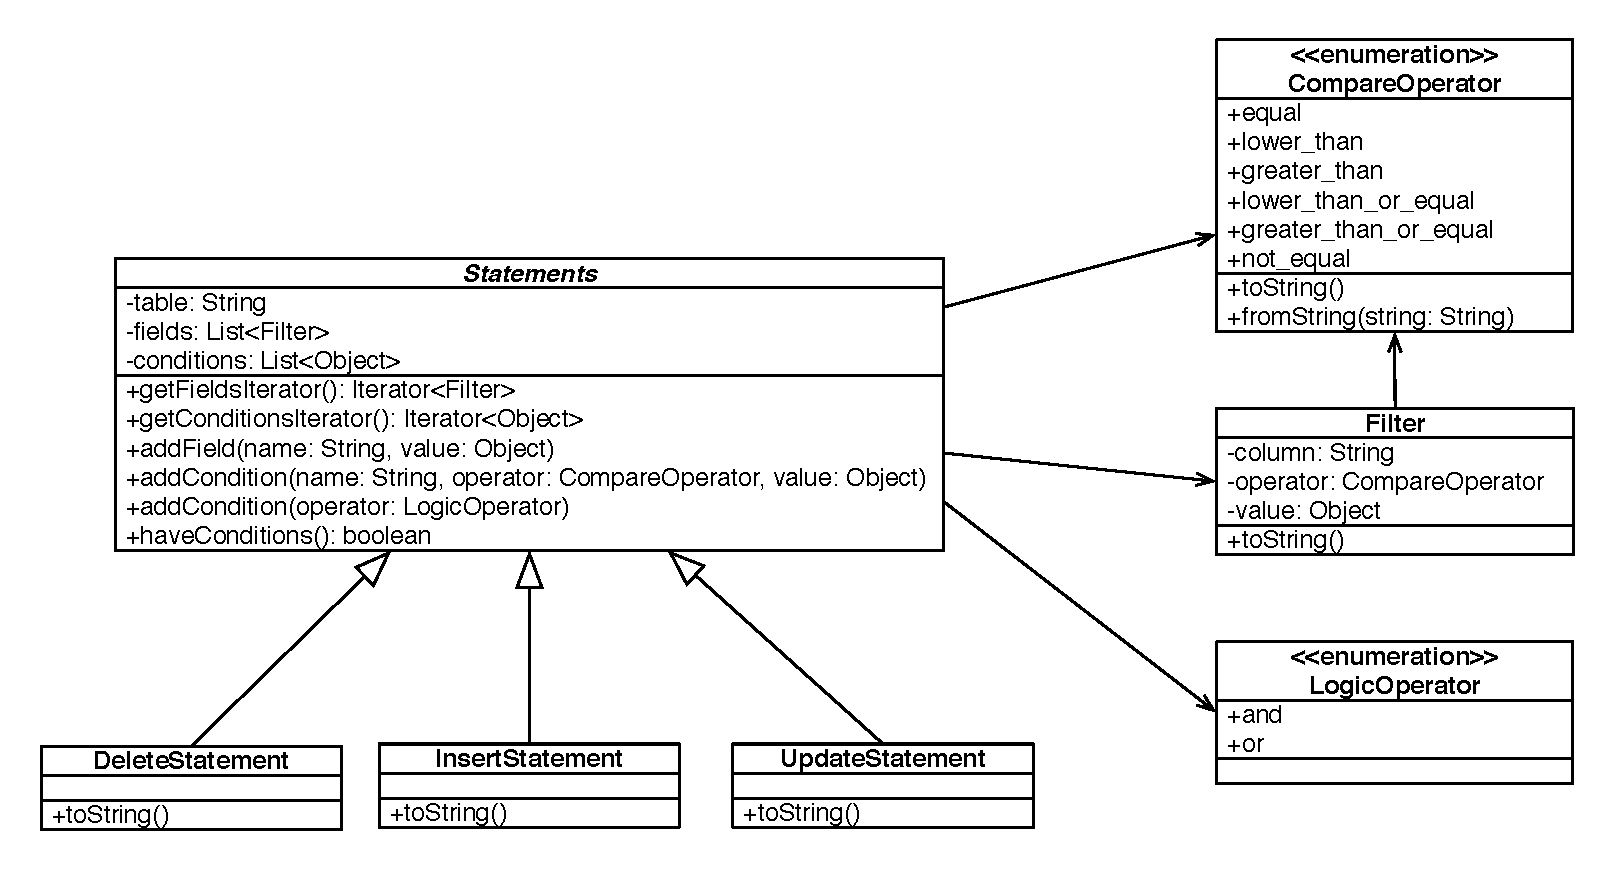
\includegraphics[width=13cm]{images/statements}
  \caption{Statements structure}
  \label{fig:statements}
\end{figure} 

\noindent The \texttt{Statement} class maintains three main fields:
\begin{itemize}
\item \texttt{table}, that contains the table which the statements refer to
\item \texttt{fields}, a list of element of class \texttt{Filter} that contains the elements presents in the \textit{SET} clause in case of \textit{UPDATE} statements or the inserted values in case of \textit{INSERT} statements
\item \texttt{conditions}, a linked list of \texttt{Filter} elements and \texttt{CompareOperator} elements, to represents the \textit{WHERE} clause 
\end{itemize} 

\noindent Since not all those elements are needed in all the statements type, specific statements implementations overrides the method that \texttt{Statements} provide for handling those fields to deny their usage. For example since the \textit{INSERT} statements does not permit a \textit{WHERE} clause, trying to add a condition to the statement will result in an \texttt{UnsupportedOperationException}. Another case is the \textit{DELETE} statements that requires only the \textit{WHERE} clause so the exception is thrown trying to add to it a \textit{field}.

\newparagraph Defined the statements structure is then necessary to provide a way to build the correct instance of statement starting by the query or the operation on an object.
To do this in an agile way a builder class has been implemented.

\begin{figure}[tbh]
  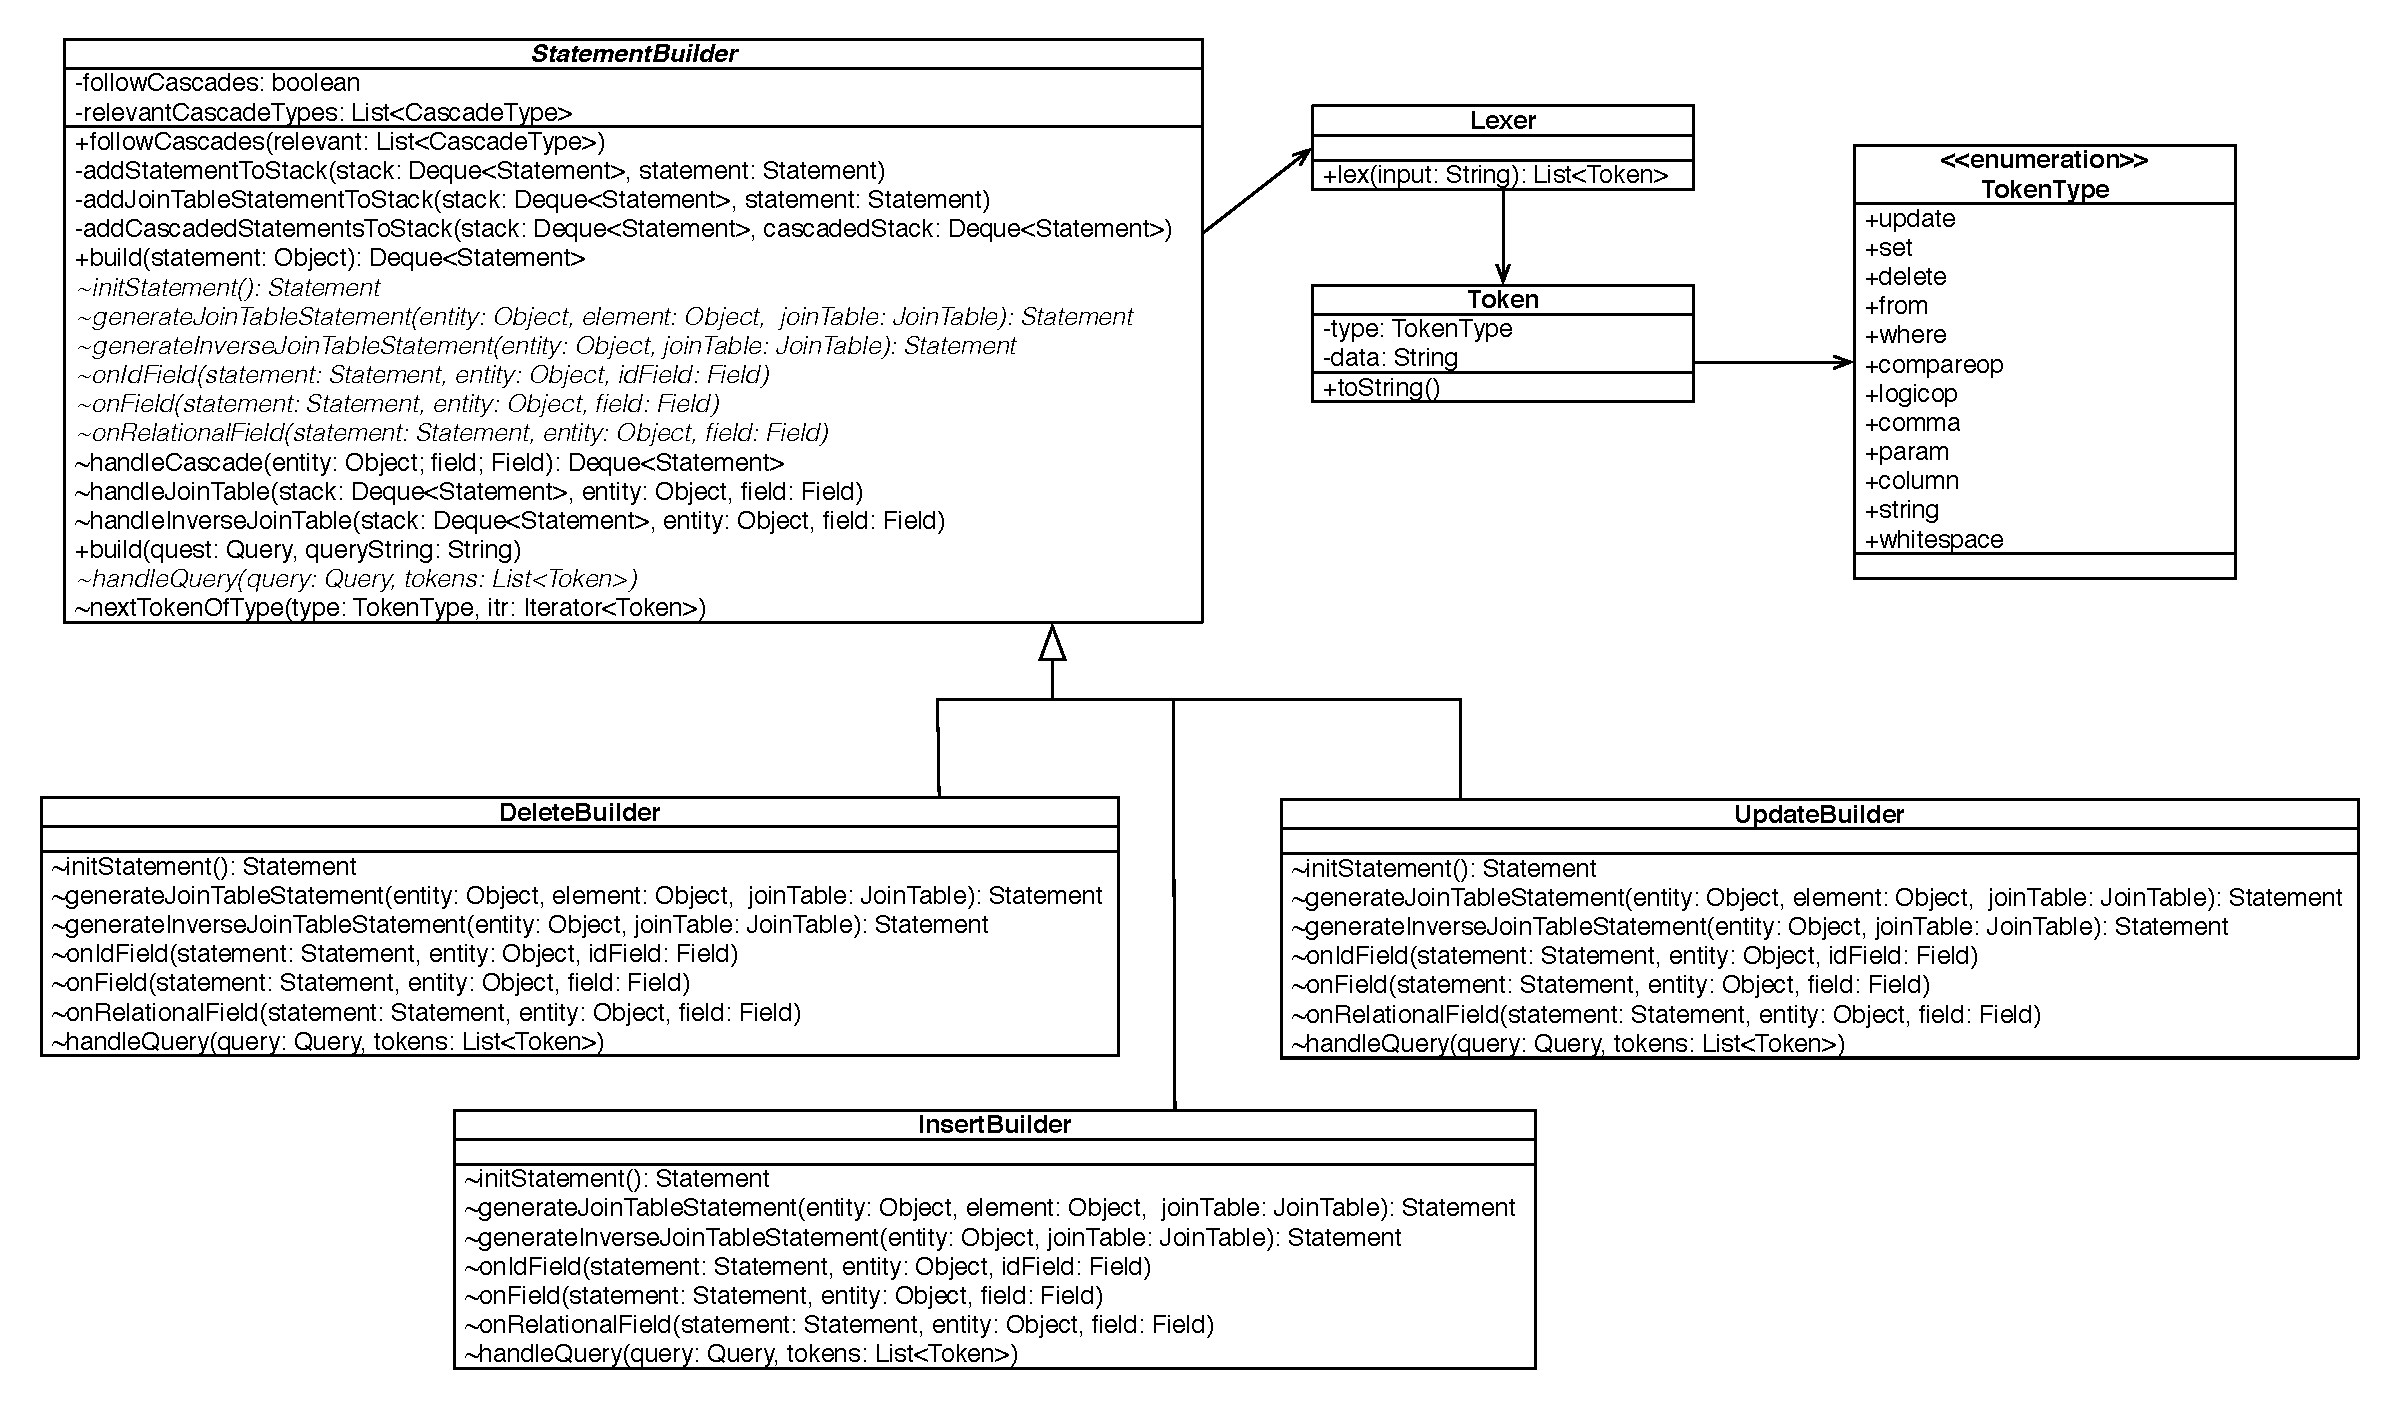
\includegraphics[width=16cm]{images/builders}
  \caption{Statement builders}
  \label{fig:builders}
\end{figure} 

\noindent The class diagram of the builders, shown in figure \ref{fig:builders}, shows that the same pattern used for statements has been adopted.

\noindent The main abstract class \texttt{StatementBuilder} provides the facilities to build a generic statements both from object and from a query string.
Since many operations are the same for all the three types of statements to be built, the \texttt{StatementBuilder} class provides an implementation of those common behaviors, and define some \textit{abstract} methods that are statement-specific and handled in different ways in the three statement builder classes: \texttt{InsertBuilder}, \texttt{UpdateBuilder} and \texttt{DeleteBuilder}.
This degree of abstraction has been possible due to the abstract definition of the \texttt{Statement} class, this allow to the \texttt{StatemetnBuilder} to acts independently from the specific statement type and then delegate to the specific builder in the cases in which such abstraction is not sufficient anymore.

\subsection{Build statements from objects}
The main problem in generating statements form objects were the cascade type. From the JPA specification \cite{book:projpa2}, the user, on relational fields, can define which type of cascade type he wants to be applied upon operations performed on the entity. The cascade type can be specified through the annotation \texttt{@CascadeType}, four are the relevant values:
\begin{itemize}
\item \texttt{PERSIST}, when the entity is persisted, every related entity is persisted too, without the need of any explicit persist for that entity
\item \texttt{MERGE}, when the entity is updated, every related entity is updated too, without the need of any explicit merge for that entity
\item \texttt{REMOVE}, when the entity is deleted, every related entity is deleted too, without the need of any explicit delete for that entity
\item \texttt{ALL}, which enclose all the previous types
\end{itemize}

\noindent The problem in supporting such operations is that statements generated by cascade must keep a logical order, for example if an entity \textit{A} is inserted and is related to another new entity \texttt{B}, the entity \texttt{B} must be inserted after the insert of the first entity. Even if it's possible to guarantee this ordering, the main problem is that the migration system cannot guarantee operation orderings since operations should be executed within a transaction.

\newparagraph Even if the migration system does not support transactions yet, has been decided to implement also the case of following the cascade types in case the migration system will be able to guarantee operation ordering in future versions.
This behavior has been made configurable, the default value can be changed through the relative voice in the \texttt{migration.xml} (see the appendix \ref{app:migration} for further details) but also at run-time by calling the appropriate methods on the class \texttt{BuildersConfiguration}. The statements builders, when created, asks to that class in order to decide if the build process should or not consider the cascade types and if its the case they set the \texttt{relevantCascadeTypes} accordingly.
The relevant cascade types has been defined as follow:
\begin{enumerate}
\item \texttt{ALL} and \texttt{PERSIST}, for \textit{INSERT} statements
\item \texttt{ALL} and \texttt{MERGE}, for \textit{UPDATE} statements
\item \texttt{ALL} and \texttt{REMOVE}, for \textit{DELETE} statements
\end{enumerate}
\noindent To define the statements ordering has been taken the ordering that should be respected as if the statements are for a SQL database, in this situation \textit{join table statements} must be taken with particular care since inserts in the join table must be happen \textbf{after} the insert of the entity itself, deletes in the join table must be happen \textbf{before} the delete of the entity itself.

\newparagraph The builder abstract class \texttt{StatementBuilder} provides a single entry point for statements building which is the method \texttt{build(Object entity)}. This method is designed following a template pattern, the designed general algorithm (reported in algorithm \ref{code:statements-building}) perform all the operations needed to   build the statement and calls several methods defined as abstract, which are implemented in the specific builders since they require specific logic, and several hook methods that can be overrided by the specific builders to change the algorithm behavior.

\begin{algorithm}[h]
  %{\footnotesize\selectfont
  \begin{algorithmic}[1]
  \Function{build}{$object$} 
    \State $stack \gets$ empty queue
    \State $cascadedStack \gets$ empty queue
	\State $statemet \gets$ \Call{initStatement}{}
    \State \Call{setTableName}{$statement$, $object$}
    \ForAll{$field \gets$ \Call{getFields}{$statment$}}
      \If{\Call{isRelational}{$field$} $\And$ \Call{ownRelation}{$field$}}
        \If{$handle$\textunderscore $cascades$}
          \State $cascadedStack \gets$ \Call{handleCascade}{$object$, $field$}
        \EndIf
        \If{\Call{isManyToMany}{$field$}}
          \State \Call{handleJoinTable}{$stack$, $entity$, $field$}
        \Else
        	  \State \Call{onRelationalField}{$statement$, $entity$, $field$}
        	\EndIf
      \Else
        \If{\Call{isManyToMany}{$field$}}
          \State \Call{handleInverseJoinTable}{$stack$, $entity$, $field$}
        	\EndIf
      \EndIf
        \If{\Call{isId}{$field$}}
          \State \Call{onIdField}{$statement$, $entity$, $field$}
        \Else
          \State \Call{onField}{$statement$, $entity$, $field$}
        \EndIf
    \EndFor        
    \State \Call {addStatementToStack}{$stack$, $statement$}
    \If{\Call{isId}{$field$}}
      \State \Call{addCascadedStatementsToStack}{$stack$, $cascadedStack$}
    \EndIf
  \EndFunction
  \end{algorithmic}
  %}	
  \caption{Template algorithm for statements building}
  \label{code:statements-building}
\end{algorithm}

\noindent Cascade generation is handled through the method \texttt{handleCascade(Object entity, Field field)} where \texttt{field} is the field of the entity that represents the related entity. The \texttt{handleCascade} method checks whenever a statements needs to be generated based on \texttt{relevantCascadeTypes} and then recursively calls \texttt{build(Object entity)} passing as \texttt{entity} the related object. 

\subsection{Build statements from JPQL queries}
Cascade modification for \textit{UPDATE} and \textit{DELETE} statements should raise if the statement, beside modifying the entity directly stated in the query, modify another related entity. Fortunately this is not a possible case for JPQL, for the object case this is possible since objects keeps reference to the related entity and if that has been modified, a cascade operation should be performed.
 
\newparagraph The main problem for JPQL queries is parsing. Since JPQL is a  object query language it make use of an object identifier on which use the dot notation to specify the object properties, furthermore JPQL allows the user to define parameter placeholders (the ones starting with ":") that are filled later through the method \texttt{setParameter(String name, Object value)} of the \texttt{Query} class.

\noindent The translation that should be performed is shown in the following snippet:

\begin{lstlisting}[language=SQL, caption=JPQL to SQL translation, label=code:query-translation, numbers=none]
# JPQL query string
UPDATE Test t SET t.name = :name WHERE t.salary >= :salary

# SQL version
UPDATE Test SET name = 'Fabio' WHERE salary >= '42'
\end{lstlisting} 

\noindent The parameter mapping can be done easily since \texttt{CloudQuery} and \texttt{TypedCloudQuery} by implementing the required JPA interfaces can intercept the \texttt{setParameter} method and so maintain the name-value mapping.

\newparagraph To solve the parsing problem, the Kundera code was inspected to understand how JPQL queries are parsed but turns out they used a custom quite-complex parser especially for validation purposes. Even looking online no specific JPQL parser has been found so, since we are not interested in validating queries or build complex logic on them, a simple and less time consuming solution was to write a lexer that through regular expressions tokenize the JPQL string.

\noindent Even the building of statements from queries follows a template pattern, the \texttt{StatementBuilder} class provides the template method \texttt{build(Query query, String queryString)} that tokenize the query using the lexer and then call the abstract method \texttt{handleQuery(query, tokens)} that is implemented in \texttt{DeleteBuilder} and in \texttt{UpdateBuilder} which are responsible of iterate over the tokes to build the correct \texttt{Statement} instance.
The \texttt{build(Query query, String queryString)} calls other various hook methods that can be overrided by the specific builders to change the algorithm behavior.

\subsection{Sending statements to Hegira}
Both the method \texttt{propagate(Query query)} and \texttt{propagate(Object entity, OperationType operation)} fill a statement stack which contains the generated statements in the execution order.

\noindent The statement stack is iterated and each time a statement is removed from the head of the stack (LIFO order). Each one of the extracted statement is then sent to \texttt{Hegira}.

%\newparagraph \textbf{TODO update when this part will be done}

\section{Interoperability of stored data}
The Kundera client developed and described in chapter \ref{chap:kundera} was developed to be as much as consistent to the other client developed for Kundera to be more likely accepted by the community and so are not built to be completely interoperable.
In an optic of data migration what we want to achieve is that data stored within a database and migrated to another one are still readable to the application without changes besides the new database configuration. 

\noindent The problem for Kundera clients are the relationships. Each database have its own ways to define identifier for the persisted entities, for Google Datastore there's the \texttt{Key} with \textit{Kind} and an \textit{identifier}, for Azure there are the \textit{partition-key} and the \textit{row-key}.Concepts are different but actually quite similar since both databases are key-value columnar database. 
A solution to the problem would have been to modify the migration system in order to make it aware of the problem and let it translate the relational columns in the format of the target database, in this way the relational columns should have been identified in some way to let the system handle them. This can be done by adding a pre-defined prefix or a suffix to those columns.
Since this solution require a good amount of changes in the migration system, other solution have been explored.
 
\newparagraph Back to the concept of identifier, generally, in columnar databases, columns are grouped in a \textit{column family} and set of columns are identified by a \textit{key}, actually the \textit{key} can span among different \textit{column families} but that's not possible either in Datastore or Azure Table.
The pair (\textit{column family}, \textit{key}) is sufficient to identify an entity (composed by one or more columns) is so needed a mapping between database-specific terminology to the more general one, this mapping is shown in table \ref{table:mapping}.

\begin{table}[h]
\begin{center}
\renewcommand{\arraystretch}{1.4}
\begin{tabular}{lcc}
\hline
\textbf{General concept} & \textbf{Datastore} & \textbf{Azure Table}\\ 
\hline\hline
Column Family & Kind & partition-key \\
Key & key-identifier & row-key \\
\hline
\end{tabular}
\end{center}
\caption{Column family and Key mapping among supported databases.}
\label{table:mapping}
\end{table}

\noindent At this point is needed a common way of save relationships as column family and key in a way that is interoperable among both the client extension.
The proposed solution is to persist \texttt{columnFamily\textunderscore key} an idea that came from the Azure Table extension which already save relationships similar to this. This solution has to be preferred w.r.t the one that require modification of the migration system since the interoperability is achieved transparently to it.

\subsection{Kundera clients modification}
Since lot of work has already been done on the Kundera clients, the modification to them has been made on a separate branch of the projects named \textit{migration}.

\paragraph{Google Datastore} The Datastore extension has been modified to persist relationships as \texttt{kind\textunderscore key-identifier} instead of the \texttt{Key} instance.
Join tables require particular care. Kundera is not providing the class of the entities involved in the join table but just the column names and the identifier (the one with the \texttt{@Id} annotation). Queries are possible even if the \textit{Kind} is unknown since Kundera provides the entity class with the entity identifier in the find operation.
To be more consistent and apply the identifier pattern (\texttt{kind\textunderscore key-identifier}) even for join tables, a map is maintained in the client and built inspecting Kundera metadata to keep track of which entity classes are involved in which many to many relationship.

\paragraph{Azure Table} The Azure Table extension has been modified too to reflect the newly defined standard for relationships. The actual problem here is that user can manually handle the partition-key but is not a possibility that can be guaranteed since if an entity is persisted with a partition-key, it will be read by the Datastore extension as of that \textit{Kind}.
Since the \texttt{Kind} in Datastore extension is the entity table name, has been decided to lock the Azure Table partition-key to the table name so user cannot decide its own since this will break the interoperability of data.
The thing to notice is that the decided pattern \texttt{partition-key\textunderscore row-key} has not been broken, the only limitation is the one that fix the partition-key to the table name.

\noindent The same discussion for the join tables made previously for Datastore applies as is also for the Azure Table extension.

\section{Summary}
In this chapter has been rapidly described the CPIM structure and the architecture of the NoSQL service before this work. Then has been described how was possible to integrate Kundera as unique persistence provider in the NoSQL service and the problem encountered in the process.

\noindent From section \ref{sec:hegira} has been described the general interaction we wanted to build to make CPIM and Hegira communicate and was then introduced and described the architecture and the design choices operated in order to develop such interaction. 
